% !TeX spellcheck = pl_PL
\newpage
\section{Wdrożenie i testowanie systemu \NazwaSys} \label{sec:testy}
Rozdział skupiać się będzie na przedstawieniu działania systemu oraz w jakim środowisku zostało testowane. Wizualizacja funkcjonowania modułów, będzie jednocześnie, krótkimi testami poprawności zaprojektowanych poszczególnych części implementacji. 

\subsection{Środowisko testowe}
Stanowisko testowe podczas implementacji projektu składa się z:
\begin{itemize*}
	\item laptopa z systemem Windows 10 EDU służącego, jako serwer (aplikacja serwerowa, baza danych),
	\item mikrokomputera Raspberry Pi 3 Model B, jako urządzenie sterujące oraz moduł zliczania osób,
	\item kamera IP Dahua DH-IPC-HDW2220RP-ZS, jako kamera zliczająca,
	\item 3 smartphony różnych modeli:
	\begin{enumerate*}
		\item Samsung S5 Neo (Android 6.0),
		\item Samsung S5 (Android 6.0),
		\item ZTE Blade A452 (Android 5.1).
	\end{enumerate*}
\end{itemize*}

Testowy laptop posiada następujące parametry:
\begin{itemize*}
	\item pamięć ram 32 GB,
	\item procesor Intel Core i7-6700HQ,
	\item dysk SSD NVMe o średniej prędkości odczytu 1,6GB/s i odczycie 920MB/s,
	\item karta graficzna Nvidia Quadro M2000M,
	\item karta sieciowa Intel Dual Band Wireless-AC 8260.
\end{itemize*}

\subsection{Wizualizacja działania systemu \textsl{\NazwaSys}}
Poniżej zostaną opisane poszczególne funkcje systemu wraz z opisem interakcji pomiędzy użytkownikiem oraz systemem. Podczas wizualizacji zakładamy żę cały system został poprawnie zainstalowany. Środowisko testowe zostało dokładnie opisane w poprzednim punkcie.

\begin{enumerate*}
	\item Logowanie (strona internetowa) \newline
	Test polegał na wykonaniu logowania błędnymi danymi (Rys. \ref{rys:Strona3} oraz sprawdzenia czy pomimo braku zalogowania można było uzyskać dostęp strony historii użycia zamków. \newline
	Wnioskiem z testów jest stwierdzenie poprawności komunikowania o błędnym logowaniu. Próbując przejść na stronę główna nie będąc zalogowany, zostajemy przekierowani do strony logowania.
\begin{figure}[ht!]
		\centering
		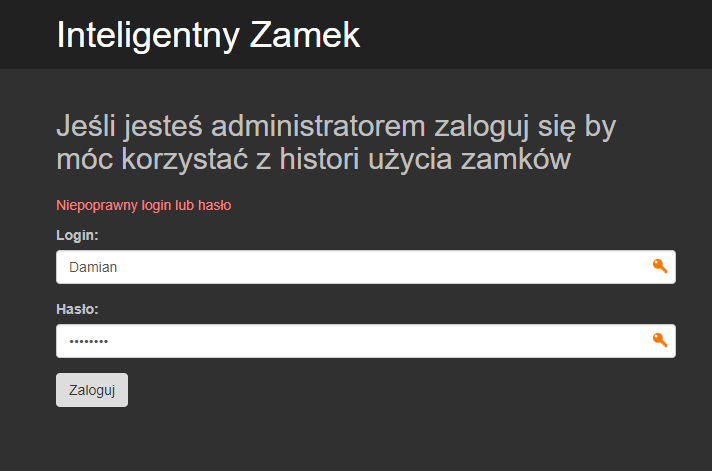
\includegraphics[width=8.5cm]{Obrazy/Strona3}
		\caption{Strona logowania -- walidacja hasła}
		\label{rys:Strona3}
\end{figure}

	\item Zliczanie osób: \newline
	 Test polegał na sprawdzeni poprawności zliczania osób w korytarzu, gdy przechodzą przez niego osoby w obie strony.
	
	Wnioski: Podczas testu wykryto prawidłową liczbę osób, które umownie ''weszły'' oraz ''wyszły''. Efekt widoczny jest na zrzutach ekranu z urządzenia sterującego. Początkowo liczniki osób wchodzących i wychodzący w lewym góry rogu ekranu wynoszą zero (Rys. \ref{rys:Kamera1}), taka sama wartość występuje przy wartości na stronie internetowej (Rys. \ref{rys:Strona1}). Rysunek \ref{rys:Kamera2} i \ref{rys:Strona2} przedstawia stan po ''wejściu'' do pomieszczenia. Działanie zliczania osób wychodzących przedstawia Rys. \ref{rys:Kamera3}.

	\begin{figure}[ht!]
		\vspace{-0.35cm}
	\begin{minipage}{0.3\textwidth}
		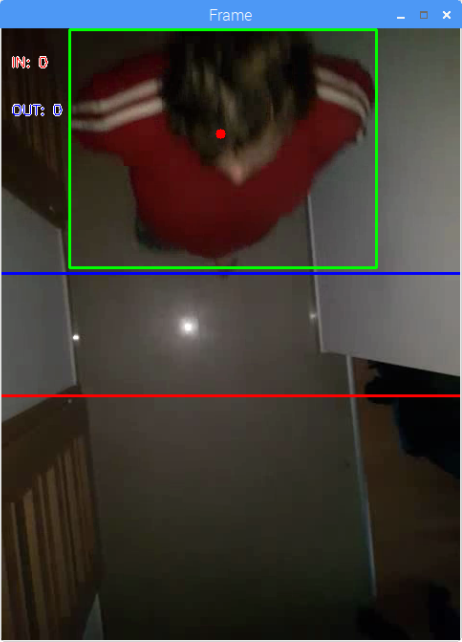
\includegraphics[width=\textwidth]{Obrazy/Kamera1}
		\caption{Stan początkowy testu zliczania osób }
		\label{rys:Kamera1}
	\end{minipage}
	\hspace{0.01\textwidth}
	\begin{minipage}{0.69\textwidth}
		\vspace{-1cm}
		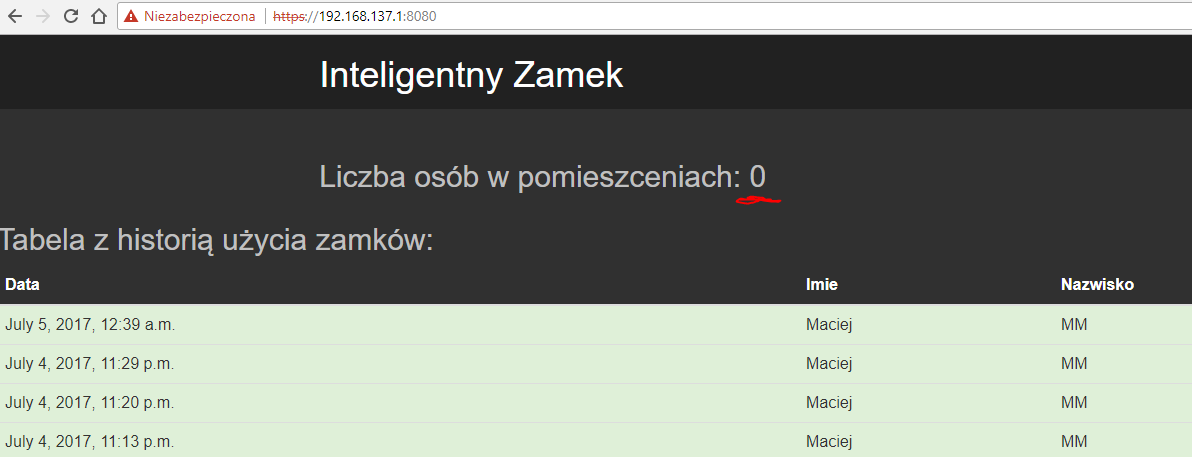
\includegraphics[width=\textwidth]{Obrazy/Strona1}
		\caption{Stan początkowy testu zliczania osób}
		\label{rys:Strona1}
	\end{minipage}
	\end{figure}

	\begin{figure}[ht!]
		\vspace{-1.5cm}
	\begin{minipage}{0.69\textwidth}
		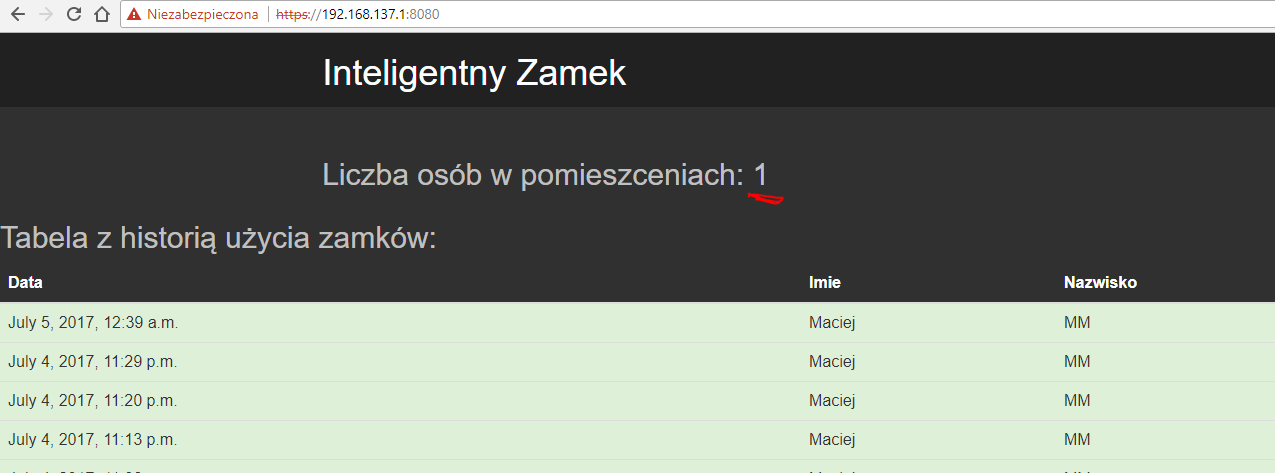
\includegraphics[width=\textwidth]{Obrazy/Strona2}
		\caption{Stan po ''wejściu'' osoby }
		\label{rys:Strona2}
	\end{minipage}
	\hspace{0.01\textwidth}
	\begin{minipage}{0.3\textwidth}
		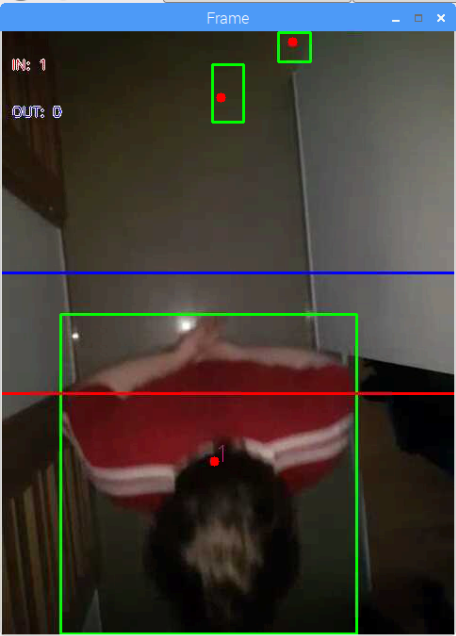
\includegraphics[width=0.9\textwidth]{Obrazy/Kamera2}
		\caption{Stan po ''wejściu'' osoby}
		\label{rys:Kamera2}
	\end{minipage}
\end{figure}

	\begin{figure}[ht!]
		\vspace{-1.7cm}
		\centering
		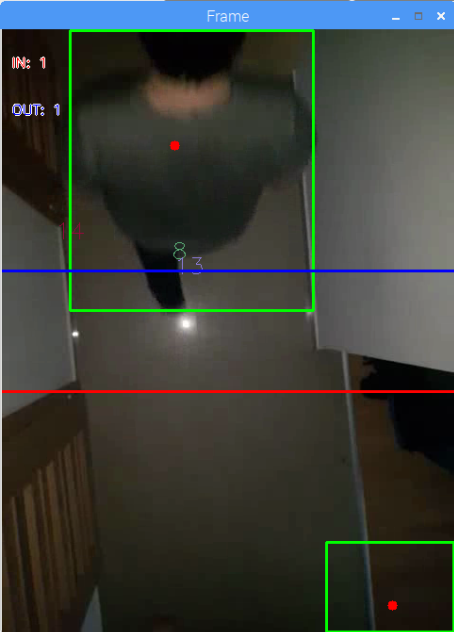
\includegraphics[width=4cm]{Obrazy/Kamera3}
		\caption{Stan po ''wyjściu'' osoby}
		\label{rys:Kamera3}
	\end{figure}
\newpage
	\item M Symulacja otwarcia
	\item M (strona) historia
	\item M logowanie użytkownika
	Walidacja hasła 
	zalogowanie, 
	opisanie panelu bocznego
	\item M rejestracja
	wyświetlanie podpowiedzi do hasła
	walidacja hasła 
	ukazywanie ukrywanie hasła
	rejestracja (komunikat +przekierowanie)
	\item M (admin)zaakceptowanie rejestracji
	widok rejestracji odrzucenie 
	akceptowanie wyniki
	\item D wnioskowanie o certyfikat
	widok wnioskowania o certyfikat
	\item D wygenerowanie nowego klucza dostępowego
	wygenerowanie nowego klucza (wnioski) 
	\item D zaakceptowanie certyfikatu dostępowego przez administratora
	akceptacja certyfikatu opusprzejscia
	\item D (admin) wygenerowanie certyfikatu dostępowego
	\item D  pobranie certyfikatu
	\item M uzyskanie dostępu do zamka (aktywacja bluetooth)
		 jako podpunkt pokazanie braku dostępu do zamka (zmiana daty)
	\item D przedłużenie certyfikatu dostępowego
	przypis bo opisane wcześniej
	\item M blokowanie certyfikatu szyfrującego *admin, user)
	\item M (admin) historia użycia zamka
	ukazanie hsitroi zamka
	\item D zarządzanie kontami użytkowników
			przypis bo wczesniej było opisane
			pod pkt zablokowanie klucza prywatnego
			przypis bo opisane wczesniej było
			pod pkt zablokowanie konta użytkownika
	\item  D eksport/import klucza
	przypis bo opisane w czesnije było
\end{enumerate*}
